\section{Data Set and Data Preprocessing}
We choose two data sets to train Neural Network, including iris and abalone.The iris data set has 150 instances, 4 features and 3 categories. And the abalone data set has 4117 instances, 8 features, and 29 categories.

\textbf{Reshuffle data set}. For each data set, we reshuffle the data set so that the model can learn more general features from it. 



\begin{figure}[tb]
	\centering
	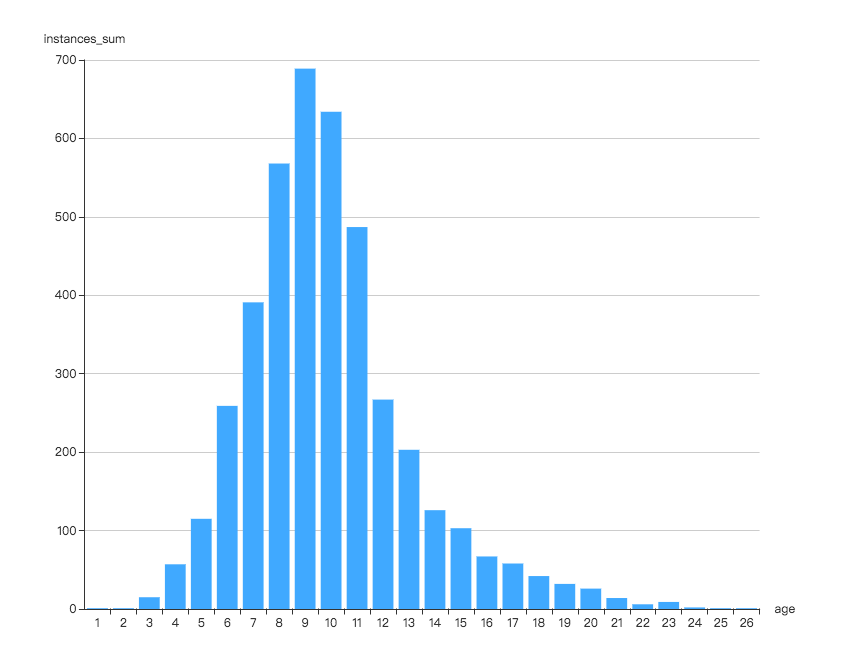
\includegraphics[width = .5\textwidth]{images/age-dis.png}
	\caption{The histogram on classification and its number of instances on abalone data set.}
	\label{fig:age-dis}
\end{figure}

\textbf{Combine different categories}. As for abalone data set, there are 29 classifications and the histogram on classification and its number of instances is show as Figure \ref{fig:age-dis}. We can see four ages including 7, 8, 9 and 10 are far higher than others. It is so imbalance between different classification that the neural network can not well classify them. So we combine different categories to three categories: lower than 9, 9 and 10, bigger than 10. 

\textbf{Split train set, validation set and test set}. And we divide data set into train set, validation set and test set by 80\%, 10\% and 10\%. As the model optimizes the learnable parameters on the training set, the loss value on the training set is gradually reduced. But when the number iterations is too big, the model will learn the features specific to this training set but not universal features. As a result, the model is overfitting and accuracy decreases.

So we use training set and validation set to train model and decide whether to early stop. At each iteration, we firstly use training data set to optimize the model with SGD algorithm and respectively calculate average loss values of training data and validation data. If the average loss values of training data or validation data increases 5 times, which means loss value on validation data set has converged and will be overfitting if continue training, we early stop the training.